\chapter{Heat Flux and Surface Temperature}

\section{NIST/NRC Test Series, Cables}

Target temperature and heat flux data are available from the NIST/NRC test series.  In the NIST/NRC tests, the targets are different types of cables in various configurations: horizontal, vertical, in trays, or free-hanging.  Figure \ref{fig:Target_Scatter} shows a comparison of predicted and measured values for radiation, total heat flux, and target temperature, along with a summary of the relative difference for the tests.

\begin{figure}[p]
\begin{center}
\begin{tabular}{lr}
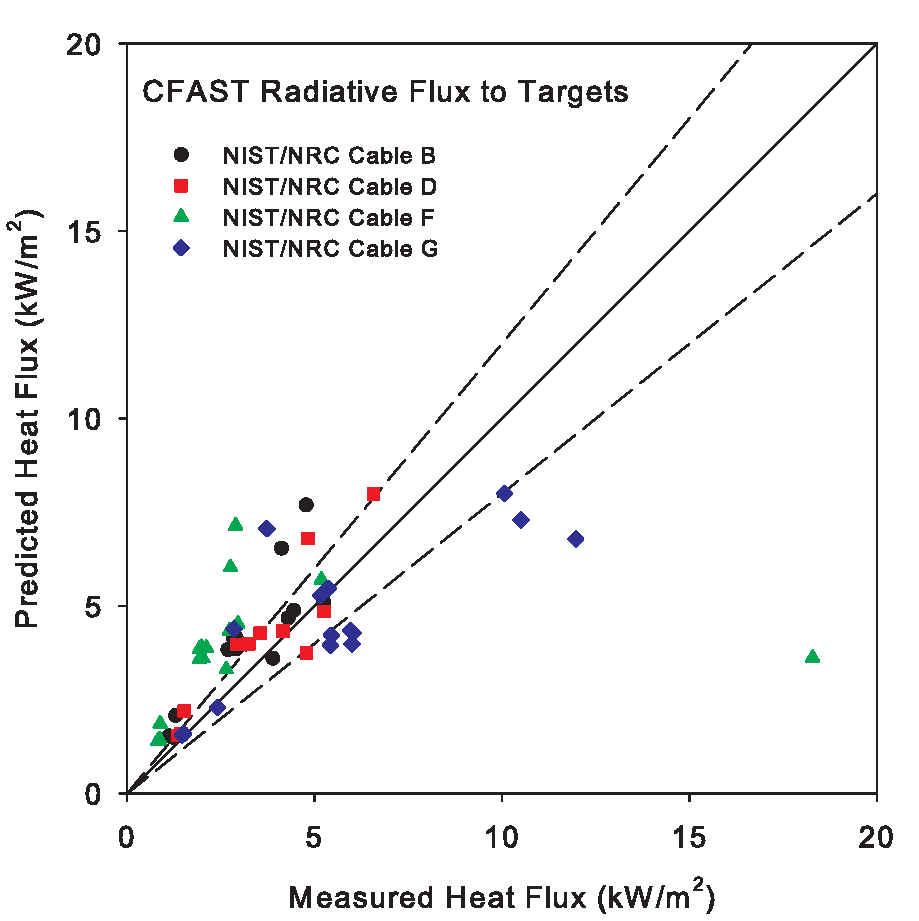
\includegraphics[width=2.6in]{FIGURES/ScatterPlots/Target_Rad} & 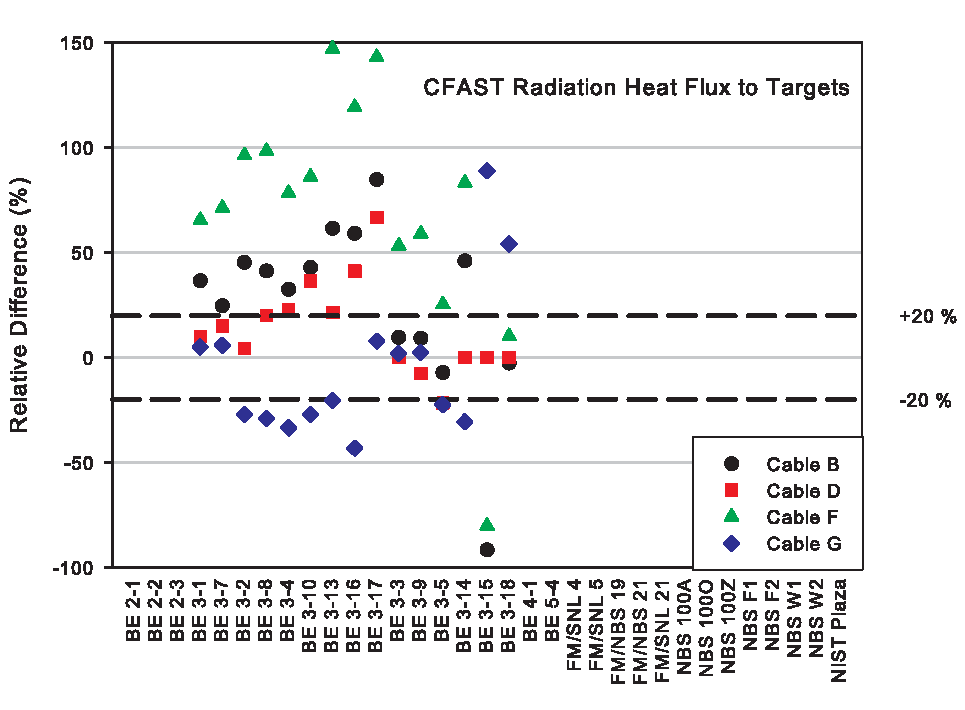
\includegraphics[width=3.5in]{FIGURES/Relative_Diff/Target_Rad}  \\
\includegraphics[width=2.6in]{FIGURES/ScatterPlots/Target_Total} & \includegraphics[width=3.5in]{FIGURES/Relative_Diff/Target_Total}  \\
\includegraphics[width=2.6in]{FIGURES/ScatterPlots/Target_Temps} & \includegraphics[width=3.5in]{FIGURES/Relative_Diff/Target_Temps}
\end{tabular}
\end{center}
\caption{Comparisons of Measured and Predicted Heat Flux to Targets and Target Temperature} \label{fig:Target_Scatter}
\end{figure}

Appendix A provides nearly 200 comparisons of heat flux and surface temperature on four different cables.  It is difficult to make sweeping generalizations about the accuracy of CFAST.  The following trends are notable:
\begin{itemize}
\item Overall, the comparisons of target flux and temperature show larger relative differences than other quantities. This is to be expected since the target flux and temperature are inherently local quantities.
\item The difference between predicted and measured cable surface temperatures is often within experimental uncertainty, with exceptions most often in the values for the vertically-oriented Cable G.  Target surface temperature predictions average within 18~\% of experimental values.  Accurate prediction of the surface temperature of the cable should indicate that the flux to the target (a combination of radiation from the fire, surrounding surfaces, and the gas layers, along with convection from the surrounding gas) should be correspondingly accurate.  For the NIST/NRC tests, the cable surface predictions show lower relative difference overall compared to the total heat flux and (particularly) the radiative heat flux.
\item Total heat flux to targets is typically predicted to within an average difference of 29~\% and often under-predicted.  Predictions for Cables D (horizontal) and G (vertical) are notable exceptions, with higher uncertainties.
\item Radiative heat flux to targets is typically over-predicted compared to experimental measurements, with higher values for closed-door tests.  For the closed-door tests, this may be a function of the over-prediction of the smoke concentration, which leads to the radiation contribution from the hot gas layer being a larger fraction of the total heat flux compared to the experimental values.
\item For many of the experiments, the convective heat flux component, taken to be the difference between the total heat flux and the radiative heat flux is seen to be higher than the values typically measured in fire experiments.
\end{itemize}


\section{NIST/NRC Test Series, Compartment Walls, Floor and Ceiling}

Thirty-six heat flux gauges were positioned at various locations on all four walls of the compartment,
plus the ceiling and floor.  Comparisons between measured and predicted heat fluxes and surface temperatures are shown
on the following pages for a selected number of locations.
Over half of the measurement points are in roughly the same relative location to the fire and hence
the measurements and predictions are similar.  For this reason, data for the east and north walls are shown
because the data from the south and west walls are comparable.  Data from the south wall is used in cases where
the corresponding instrument on the north wall failed, or in cases where the fire is positioned close to the south wall.
For each test, eight locations are used for comparison, two on the long (mainly north) wall,
two on the short (east) wall, two on the floor, and two on the ceiling.  Of the two locations for each panel,
one is considered in the far-field, relatively remote from the fire; one is in the near-field,
relatively close to the fire.  How close or far varies from test to test, depending on the availability of working flux gauges.
The two short wall locations are equally remote from the fire; thus, one location is in the lower layer, one in the upper.

Figure \ref{fig:Target_Scatter} shows a comparison of predicted and measured values for radiation, total heat flux, and target temperature, along with a summary of the relative difference for the tests.

\begin{figure}[p]
\begin{center}
\begin{tabular}{lr}
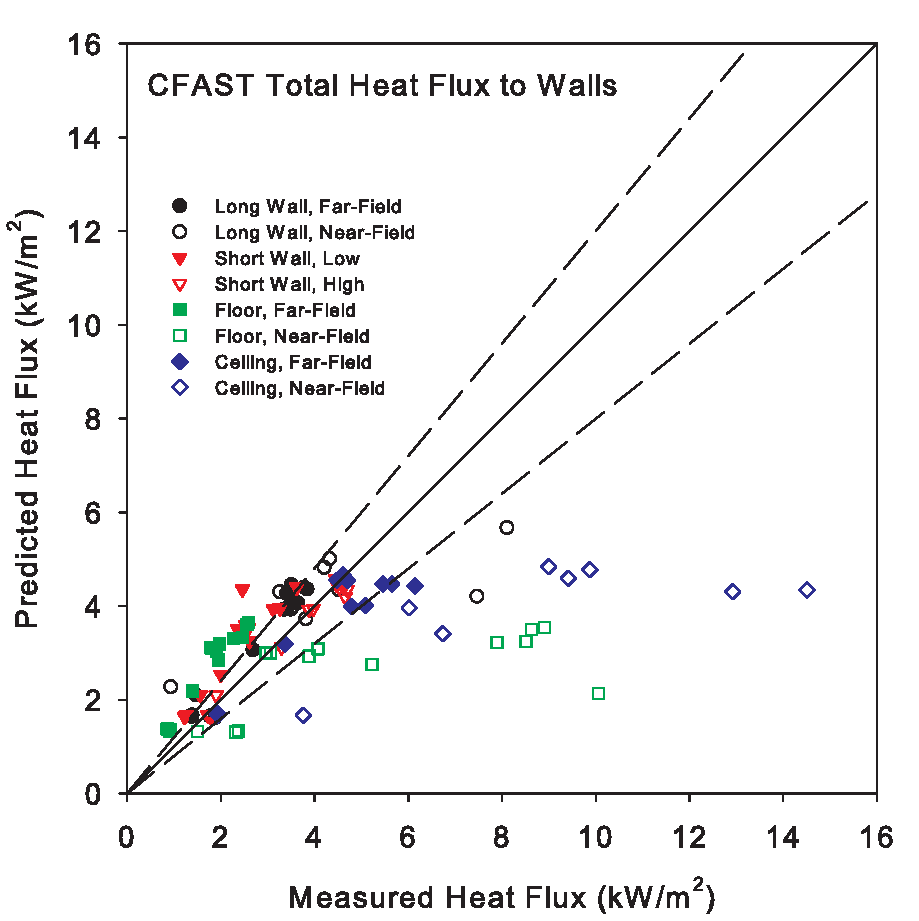
\includegraphics[width=2.6in]{FIGURES/ScatterPlots/Wall_Total} & 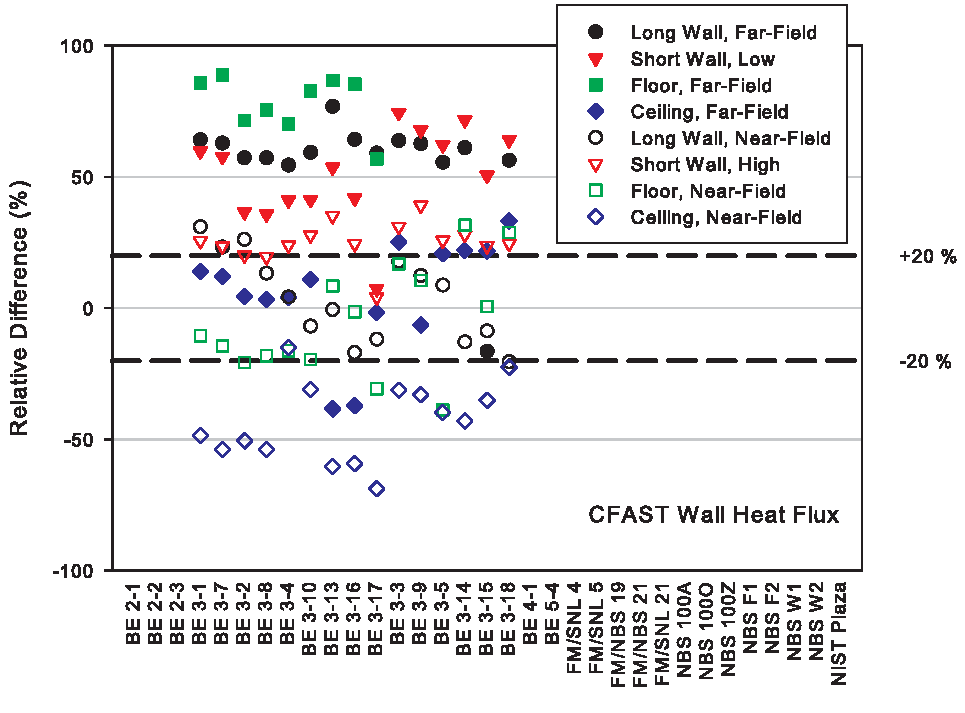
\includegraphics[width=3.5in]{FIGURES/Relative_Diff/Wall_Total} \\
\includegraphics[width=2.6in]{FIGURES/ScatterPlots/Wall_Temps} & \includegraphics[width=3.5in]{FIGURES/Relative_Diff/Wall_Temps}
\end{tabular}
\end{center}
\caption{Comparisons of Measured and Predicted Heat Flux to Compartment Surfaces and Surface Temperature} \label{fig:Surface_Scatter}
\end{figure}

CFAST predicts the heat flux and surface temperature of the compartment walls to within 31~\% and 46~\%, respectively.  Typically, CFAST over-predicts the far-field fluxes and temperatures and under-predicts the near-field measurements.  This is understandable, given that any two-zone model predicts an average representative value of gas temperature in the upper and lower regions of a compartment.  Thus, the values predicted by CFAST should be an average of values near the fire and those farther away.

However, differences for the ceiling and (particularly) floor fluxes and temperatures are higher, with a more pronounced difference between the near-field and far-field comparisons.  In addition to the limitations of the two-zone assumption, calculations of the flux to ceiling and floor surfaces are further confounded by the simple point-source calculation of radiation exchange in CFAST for the fire source.  In CFAST, the fire is assumed to be a point source of energy located at the base of the fire rather than a three-dimensional flame surface radiating to surroundings.  With the fire typically at the floor surface, this makes the calculation of flux to the floor surface inherently less accurate than for other surfaces.

\section{Summary}

Use of CFAST for heat flux and temperature requires caution for the following reasons:

\begin{itemize}
\item  Prediction of heat flux to targets and target surface temperature is largely dependent on local conditions surrounding the target.  Like any two-zone model, CFAST predicts an average representative value of gas temperature in the upper and lower regions of a compartment.  In addition, CFAST does not directly predict plume temperature or its effects on targets that may be within a fire plume.  Thus, CFAST can be expected to under-predict values near a fire source, and over-predict values for targets remote from a fire.
\item Cable target surface temperature predictions are often within experimental uncertainty, with exceptions, particularly for Cables F and G.
\item Total heat flux to targets is typically predicted to within about 30~\%, and often under-predicted.
\item Radiative heat flux to targets is typically over-predicted compared to experimental measurements, with higher relative difference values for closed-door tests.
\item CFAST is capable of predicting the surface temperature of a wall, assuming that its composition is fairly uniform and its thermal properties are well-characterized.  Predictions are typically within 10~\% to 30~\%.  Generally, CFAST over-predicts the far-field fluxes and temperatures, and under-predicts the near-field measurements.  This is consistent with the single representative layer temperature assumed by zone fire models.
\item CFAST predictions of floor heat flux and temperature are particularly problematic because of the simple point-source calculation of radiative exchange between the fire and compartment surfaces.
\end{itemize}

